\documentclass[11pt,a4paper]{article}
\usepackage[T1]{fontenc}
\usepackage[margin=2.3cm]{geometry}
\usepackage{amsmath,amssymb}
\usepackage{graphicx}
\usepackage[dvipsnames]{xcolor}
\usepackage{enumitem}
\usepackage[colorlinks=true,linkcolor=blue,urlcolor=blue]{hyperref}
\setlength{\parskip}{0.6em}
\setlength{\parindent}{0pt}
\begin{document}

\begin{center}{\LARGE\bfseries openretainingwall}\\[0.4em]{\large Check a retaining wall against sliding and overturning, in three sessions.}\\[0.2em]\small PAN IIT OSS explainer \textbullet{} diploma / undergraduate to advanced undergraduate (levels 5-6)\end{center}

\section*{Why this exists}
Soil holds itself up only by friction, so wherever the ground level changes quickly it pushes sideways on whatever holds it back. This explainer shows the mathematics of that push and of the checks that engineers make for a simple gravity wall, using only areas of triangles, moments and a little trigonometry.

\section*{The end goal}
Check a retaining wall against sliding and overturning. The end goal is to check a retaining wall against sliding and overturning: compute the earth and water push, the weight and friction of the wall, the safety factors and the base pressure, and understand why drainage matters. It is a teaching model and must never be used for a real wall.

\section*{How the three sessions build up}
\begin{enumerate}[nosep]
\item \textbf{Session 1: Soil pushes, the wall must not slide or tip} (Level 1, conceptual interactive model, 60 min).
\item \textbf{Session 2: Rankine earth pressure: how hard does the soil push?} (Level 2, mathematical engineering model, 75 min).
\item \textbf{Session 3: Sliding, overturning, the middle third and water} (Level 3, simulation and validation, 90 min).
\end{enumerate}

\section{Session 1: Soil pushes, the wall must not slide or tip}

\subsection*{A. Real-world problem}
A garden bed behind a low wall looks calm, but the soil is like a heavy crowd leaning on a fence: it wants to spread out sideways. The deeper the soil, the harder it pushes, so a tall wall faces much more than a short one. The wall can fail in two simple ways: the whole wall can slide along the ground, or it can tip over its front bottom edge, the toe. How strong must a wall of a given width be?

\subsection*{B. Concept and theory}
The sideways pressure of the soil is zero at the surface and grows in a straight line with depth, so the pressure on the wall back is a triangle. The force is the area of that triangle. In this session we use a push factor Ka = 1/3 (Session 2 explains where it comes from), a soil unit weight of 18 kN/m\textasciicircum{}3 and a wall height H, which gives a push per metre of wall of 0.5 x (1/3) x 18 x H\textasciicircum{}2, acting one third of the way up. The wall is a concrete rectangle of width B and weighs 24 x B x H per metre; friction under the base resists sliding with a coefficient of 0.5. Sliding ratio = friction / push. Tipping ratio = (weight x B/2) / (push x H/3): the turning effect that keeps the wall down divided by the turning effect that tips it, both about the toe. A ratio below 1 means failure; engineers want a margin of at least about 1.5 for sliding and 2 for tipping (commonly used guidance, not a code).

\begin{itemize}[nosep]
\item H: wall height (retained soil height) (m)
\item B: wall width at the base (m)
\item P: total sideways push of the soil per metre run of wall (kN/m)
\item W: wall weight per metre run (kN/m)
\item gamma: soil unit weight (18) (kN/m\textasciicircum{}3)
\item Ka: push factor (1/3 here) (no unit)
\item mu: friction coefficient under the base (0.5) (no unit)
\end{itemize}

\begin{equation*}
P=\tfrac12 K_a\gamma H^2,\qquad \text{acts at } H/3 \text{ above the base}
\end{equation*}

\begin{equation*}
W=\gamma_c B H
\end{equation*}

\begin{equation*}
\text{sliding ratio}=\frac{\mu W}{P},\qquad \text{tipping ratio}=\frac{W\,B/2}{P\,H/3}
\end{equation*}

\begin{center}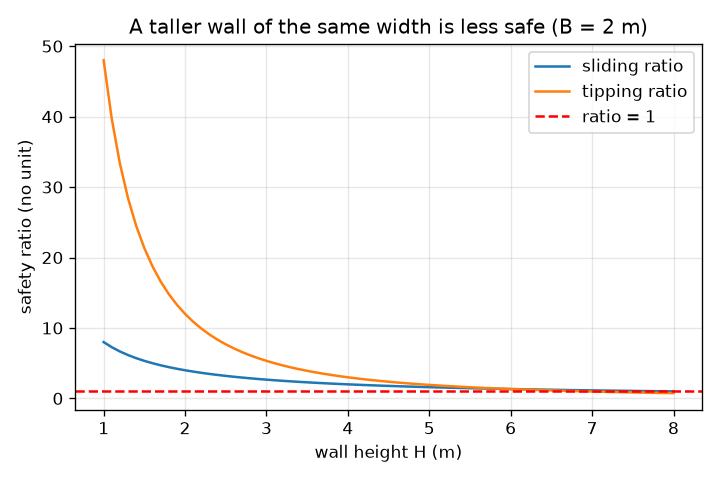
\includegraphics[width=0.85\linewidth]{figures/s01_ratio_vs_height.png}\\\small Sliding and tipping ratios against wall height for a 2 m wide wall: both fall as the wall gets taller.\end{center}

\subsection*{E. Worked example}
A wall 4 m high and 2 m wide holds dry soil. Find the push, the weight, the sliding ratio and the tipping ratio.
\begin{enumerate}[nosep]
\item Push P = 0.5 x (1/3) x 18 x 4\textasciicircum{}2 = 0.5 x 0.3333 x 18 x 16 = 48 kN/m, acting 4/3 = 1.33 m above the base.
\item Weight W = 24 x 2 x 4 = 192 kN/m, acting 1 m from the toe.
\item Sliding: friction = 0.5 x 192 = 96 kN/m, so the ratio is 96 / 48 = 2.00.
\item Tipping: resisting turning effect = 192 x 1 = 192 kN m/m; tipping turning effect = 48 x 1.333 = 64 kN m/m; the ratio is 192 / 64 = 3.00.
\end{enumerate}
\textbf{Answer.} Push 48 kN/m, weight 192 kN/m, sliding ratio 2.00, tipping ratio 3.00. Both are above the guidance values of 1.5 and 2.

\subsection*{F. Questions}
\begin{enumerate}[nosep]
\item \textbf{Conceptual.} Why does doubling the height of the soil quadruple the push on the wall, but only double the weight of a wall of the same width?
\item \textbf{Numerical.} A wall 3 m high and 1.2 m wide holds dry soil (same values as in the lesson). Find the sliding ratio and the tipping ratio. Does it meet the guidance of 1.5 and 2?
\item \textbf{Graph and simulation interpretation.} In the graph for a 2 m wide wall, at what heights do the two ratios reach 1? Which failure comes first as the wall gets taller?
\item \textbf{Design and optimisation challenge.} Design: for a 3 m high wall choose the smallest width, in steps of 0.05 m, that gives a sliding ratio of at least 1.5 and a tipping ratio of at least 2. Which ratio decides?
\end{enumerate}

\section{Session 2: Rankine earth pressure: how hard does the soil push?}

\subsection*{A. Real-world problem}
A 4 m high wall holds back dry soil. How large is the sideways push, per metre of wall, and where does it act? What changes when a parked car adds weight on the soil, or when heavy rain fills the backfill with water? And how sure can we be of the answer when the friction angle of the soil is only roughly known?

\subsection*{B. Concept and theory}
The Rankine theory treats a smooth vertical wall and level backfill. When the wall moves slightly away from the soil, the soil reaches its active state and the horizontal pressure at depth z is p = Ka x gamma x z. The coefficient Ka depends only on the soil friction angle phi: Ka = tan\textasciicircum{}2(45 - phi/2), which equals (1 - sin phi) / (1 + sin phi). For phi = 30 degrees, Ka = 1/3. The pressure is a triangle, so the resultant per metre of wall is its area, Pa = 0.5 Ka gamma H\textasciicircum{}2, acting at H/3 above the base. A uniform surcharge q on the ground adds a constant pressure Ka q, a rectangle, so a force Ka q H at H/2. Water in the backfill pushes with the full hydrostatic pressure gamma\_w z whatever the soil; for a backfill saturated to the top the soil's effective weight drops to gamma\_sat - gamma\_w and the water adds 0.5 gamma\_w H\textasciicircum{}2. Water is a warning: with gamma\_sat = 20 kN/m\textasciicircum{}3 it more than doubles the push on a 4 m wall.

\begin{itemize}[nosep]
\item phi: soil friction angle (degrees)
\item Ka: Rankine active earth pressure coefficient (no unit)
\item gamma: soil unit weight (kN/m\textasciicircum{}3)
\item z: depth below the soil surface (m)
\item p: horizontal earth pressure (kPa (kN/m\textasciicircum{}2))
\item Pa: resultant active force per metre run of wall (kN/m)
\item q: uniform surcharge on the ground (kPa)
\item gamma\_w: unit weight of water (9.81) (kN/m\textasciicircum{}3)
\end{itemize}

\begin{equation*}
K_a=\tan^2\!\left(45^\circ-\tfrac{\varphi}{2}\right)=\frac{1-\sin\varphi}{1+\sin\varphi}
\end{equation*}

\begin{equation*}
p(z)=K_a\gamma z,\qquad P_a=\tfrac12 K_a\gamma H^2\ \text{at } H/3
\end{equation*}

\begin{equation*}
P_q=K_a\,q\,H\ \text{at } H/2
\end{equation*}

\begin{equation*}
P_w=\tfrac12\gamma_w H^2,\qquad P_{soil}=\tfrac12 K_a(\gamma_{sat}-\gamma_w)H^2
\end{equation*}

\begin{center}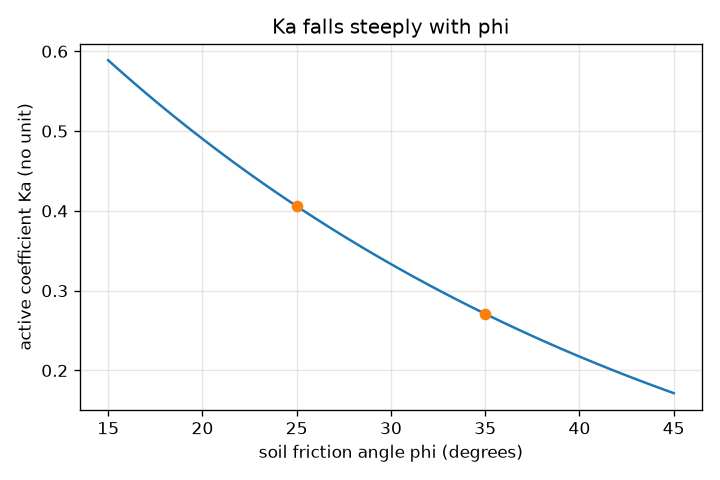
\includegraphics[width=0.85\linewidth]{figures/s02_ka_vs_phi.png}\\\small Ka against the friction angle: the dots show phi = 25 and 35 degrees.\end{center}

\subsection*{E. Worked example}
A wall 4 m high holds dry soil with gamma = 18 kN/m\textasciicircum{}3 and phi = 30 degrees. Find Ka, the pressure at the base, the force per metre and where it acts. Then add a 10 kPa surcharge.
\begin{enumerate}[nosep]
\item Ka = (1 - sin 30) / (1 + sin 30) = 0.5 / 1.5 = 1/3. The other form tan\textasciicircum{}2(45 - 15) = tan\textasciicircum{}2(30) = 0.5774\textasciicircum{}2 = 0.3333 agrees.
\item Pressure at the base = Ka x gamma x H = (1/3) x 18 x 4 = 24 kPa.
\item Force Pa = 0.5 x 24 kPa x 4 m = 48 kN/m, acting 4/3 = 1.33 m above the base.
\item Surcharge force = Ka q H = (1/3) x 10 x 4 = 13.33 kN/m, acting at 2 m.
\item Total = 48 + 13.33 = 61.33 kN/m. Its height = (48 x 1.333 + 13.33 x 2) / 61.33 = (64 + 26.67) / 61.33 = 1.48 m.
\end{enumerate}
\textbf{Answer.} Ka = 1/3, base pressure 24 kPa, Pa = 48 kN/m acting 1.33 m above the base; with a 10 kPa surcharge the total is 61.33 kN/m acting 1.48 m above the base.

\subsection*{F. Questions}
\begin{enumerate}[nosep]
\item \textbf{Conceptual.} Why is the earth pressure on a wall a triangle, and why does the resultant act at H/3 above the base rather than at mid-height?
\item \textbf{Numerical.} A wall 3 m high holds soil with gamma = 19 kN/m\textasciicircum{}3 and phi = 30 degrees. Find Pa and the height at which it acts.
\item \textbf{Graph and simulation interpretation.} From the graph of Ka against phi, what happens to Ka when phi rises from 25 to 35 degrees? What does this mean for the 4 m wall's push?
\item \textbf{Design and optimisation challenge.} Design: the wall may carry at most 60 kN/m of soil force. Find the tallest wall for gamma = 18 kN/m\textasciicircum{}3 and phi = 30 degrees, first without and then with a 10 kPa surcharge. Which is the stronger limit?
\end{enumerate}

\section{Session 3: Sliding, overturning, the middle third and water}

\subsection*{A. Real-world problem}
A small wall holds up a bed of soil. It must not slide, must not tip over its toe, and the pressure under its base must stay compressive, so that it does not try to lift off the ground at the heel. Rain can make all of this much worse: poorly drained soil fills with water that pushes on the wall and lifts the base. How wide must the wall be, and how much does bad drainage cost?

\subsection*{B. Concept and theory}
Per metre run of a rectangular gravity wall of height H and width B (weight W = gamma\_c B H at B/2 from the toe) the soil force Pa acts at H/3 (Rankine, Session 2). With a backfill rising at angle beta, the Rankine force is parallel to the slope, with a horizontal part Pa cos(beta) and a vertical part Pa sin(beta) acting on the wall back. Water at height hw above the base adds hydrostatic push and an uplift under the base that varies from gamma\_w hw at the heel to zero at the toe. Passive resistance of the soil in front of the toe is neglected, which is safe-sided. Sliding: FS\_slide = mu N / Ph, where N is the net vertical force on the base. Overturning about the toe: FS\_ot = M\_resisting / M\_overturning. The vertical resultant acts at x = (M\_res - M\_ot)/N from the toe, so the eccentricity from the base centre is e = B/2 - x. If e \textless{}= B/6 (the resultant is inside the middle third) the base pressure q = (N/B)(1 +- 6e/B) is compressive everywhere; if e \textgreater{} B/6 the heel pressure is negative (tension, which soil cannot provide). Commonly used guidance, not a code: FS\_slide at least about 1.5 and FS\_ot at least about 2.0. Coulomb theory allows a rough or leaning wall (wall friction delta, wall inclination alpha): Ka = cos\textasciicircum{}2(phi - alpha) / (cos\textasciicircum{}2(alpha) cos(alpha + delta) [1 + sqrt(sin(phi + delta) sin(phi - beta) / (cos(alpha + delta) cos(alpha - beta)))]\textasciicircum{}2). It reduces to Rankine when delta = alpha = beta = 0, which the checkpoint verifies.

\begin{itemize}[nosep]
\item B: base width of the wall (m)
\item H: wall height (4 m in the lesson) (m)
\item W: wall weight per metre run (gamma\_c B H) (kN/m)
\item Ph: horizontal force on the wall back (kN/m)
\item U: uplift force under the base (kN/m)
\item N: net vertical force on the base (kN/m)
\item mu: friction coefficient under the base (no unit)
\item e: eccentricity of the resultant from the base centre (m)
\item q: pressure under the base (toe, heel) (kPa)
\item hw: water level above the base (m)
\item beta: backfill slope angle (degrees)
\end{itemize}

\begin{equation*}
K_a=\cos\beta\,\frac{\cos\beta-\sqrt{\cos^2\beta-\cos^2\varphi}}{\cos\beta+\sqrt{\cos^2\beta-\cos^2\varphi}}
\end{equation*}

\begin{equation*}
FS_{slide}=\frac{\mu N}{P_h},\qquad FS_{ot}=\frac{M_{res}}{M_{ot}}
\end{equation*}

\begin{equation*}
x=\frac{M_{res}-M_{ot}}{N},\qquad e=\frac B2-x,\qquad e\le\frac B6\ \text{(middle third)}
\end{equation*}

\begin{equation*}
q_{toe,heel}=\frac NB\left(1\pm\frac{6e}{B}\right)
\end{equation*}

\begin{center}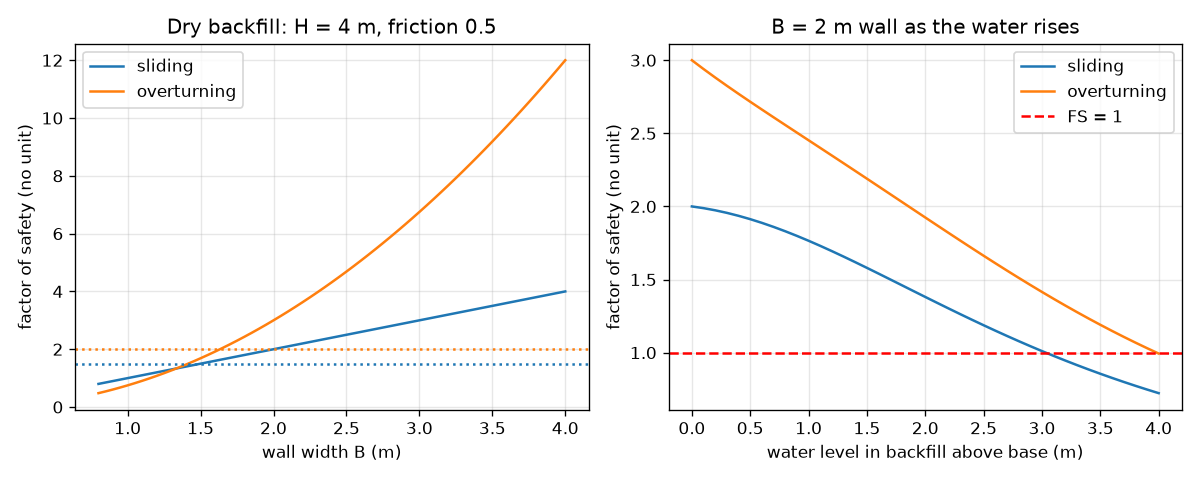
\includegraphics[width=0.85\linewidth]{figures/s03_safety_factors.png}\\\small Left: safety factors against wall width (dry). Right: a 2 m wide wall as the water rises: both factors fall through their limits.\end{center}

\subsection*{E. Worked example}
A wall 4 m high and 2 m wide (concrete 24 kN/m\textasciicircum{}3) holds dry soil (gamma = 18 kN/m\textasciicircum{}3, phi = 30 degrees), with base friction 0.5. Find both factors of safety, the eccentricity and the base pressures. Then fill the backfill with water to the top.
\begin{enumerate}[nosep]
\item Pa = 0.5 x (1/3) x 18 x 16 = 48 kN/m at 1.33 m, so M\_ot = 48 x 1.333 = 64 kN m/m. W = 24 x 2 x 4 = 192 kN/m, M\_res = 192 x 1 = 192 kN m/m.
\item FS\_slide = 0.5 x 192 / 48 = 2.00. FS\_ot = 192 / 64 = 3.00. Both are above 1.5 and 2.0.
\item x = (192 - 64) / 192 = 0.667 m from the toe, so e = 1.0 - 0.667 = 0.333 m, exactly B/6 = 0.333 m: the resultant is at the edge of the middle third.
\item q\_toe = (192 / 2) x (1 + 6 x 0.333 / 2) = 96 x 2 = 192 kPa and q\_heel = 96 x (1 - 1) = 0.
\item Saturated to the top: soil 27.17 kN/m plus water 78.48 kN/m give Ph = 105.65 kN/m. Uplift U = 0.5 x 9.81 x 4 x 2 = 39.24 kN/m acting 2B/3 = 1.33 m from the toe.
\item M\_ot = 105.65 x 1.333 + 39.24 x 1.333 = 193.19 kN m/m, so FS\_ot = 192 / 193.19 = 0.994. FS\_slide = 0.5 x (192 - 39.24) / 105.65 = 0.72.
\end{enumerate}
\textbf{Answer.} Dry: FS\_slide 2.00, FS\_ot 3.00, e = 0.333 m = B/6, toe pressure 192 kPa and heel pressure 0. Saturated: FS\_slide 0.72 and FS\_ot 0.994, both below 1, so the wall slides and tips.

\subsection*{F. Questions}
\begin{enumerate}[nosep]
\item \textbf{Conceptual.} Why does water in the backfill reduce both the sliding and the overturning factors, and why is drainage behind a wall so important?
\item \textbf{Numerical.} A wall 3 m high and 1.6 m wide (concrete 24 kN/m\textasciicircum{}3) holds dry soil (gamma = 18, phi = 30 degrees), base friction 0.5. Find FS\_slide, FS\_ot, the eccentricity and whether the resultant is in the middle third.
\item \textbf{Graph and simulation interpretation.} In the right panel of the first figure (a 2 m wide wall), at what water levels does the sliding factor fall below 1.5 and 1? At what level does the overturning factor fall below 2 and 1? Which factor fails first?
\item \textbf{Design and optimisation challenge.} Design: for a 4 m wall with base friction 0.5 (phi = 30 degrees), find the smallest width in steps of 0.05 m that passes all three checks (FS\_slide \textgreater{}= 1.5, FS\_ot \textgreater{}= 2.0, e \textless{}= B/6) for a dry backfill, and with water 2 m deep. Discuss the cost of poor drainage.
\end{enumerate}

\section{Real-world mini-project}
\textbf{Size the base width of a small garden wall.} A garden wall holds up a 1.2 m high bed of soil (unit weight 18 kN/m\textasciicircum{}3, friction angle 30 degrees). The wall is masonry with unit weight 22 kN/m\textasciicircum{}3, friction under the base is 0.45, and a 5 kPa surcharge covers people sitting on the bed. Use \texttt{wall\_state} and \texttt{min\_width} from Session 3 to find the smallest base width (in steps of 0.05 m) that gives FS\_slide of at least 1.5, FS\_ot of at least 2.0 and a resultant inside the middle third. Then repeat with water standing 0.6 m and 1.2 m deep behind the wall to see what bad drainage costs.

\section{The path ahead}
\begin{enumerate}[nosep]
\item \textbf{Session 4: Cantilever wall with a heel slab.} A wall made of a stem and a base slab, with the weight of soil on the heel included.
\item \textbf{Session 5: Passive resistance and a shear key.} A passive force at the toe and a key under the base added to the sliding check.
\item \textbf{Session 6: A drain that saves the wall.} A drainage model that sets the effective water level behind the wall from rain and drain capacity.
\item \textbf{Session 7: Bearing capacity of the ground.} A check of the toe pressure against an allowable bearing pressure.
\item \textbf{Session 8: Earthquake loading.} A function Kae for a horizontal acceleration coefficient and a check of the wall under it.
\end{enumerate}

\section{Answers and hints}

\subsection*{Session 1}
\begin{enumerate}[nosep]
\item \textbf{Conceptual.} Hint: The push is the area of a triangle whose base and height both grow with H. The weight is width times height. Solution: The pressure at the bottom doubles (it is proportional to depth) and the loaded height doubles, so the triangle's area is four times larger: 48 kN/m becomes 192 kN/m. The wall weight W = 24 x B x H only has one factor of H, so it doubles. That is why a taller wall of the same width is much less safe.
\item \textbf{Numerical.} Hint: P = 0.5 x (1/3) x 18 x 9 = 27 kN/m acting at 1 m; W = 24 x 1.2 x 3. Solution: W = 86.4 kN/m. Sliding ratio = 0.5 x 86.4 / 27 = 1.60. Tipping ratio = 86.4 x 0.6 / (27 x 1) = 51.84 / 27 = 1.92. Sliding meets 1.5, but the tipping ratio 1.92 is just below 2, so the wall is slightly too narrow.
\item \textbf{Graph and simulation interpretation.} Hint: Read where each curve touches the red line. Closed forms: sliding ratio = 4B/H, tipping ratio = 12 B\textasciicircum{}2 / H\textasciicircum{}2. Solution: The tipping ratio reaches 1 at H = sqrt(48) = 6.93 m and the sliding ratio at H = 8 m. As the wall gets taller, tipping fails first, at about 6.9 m. In practice the guidance values 1.5 and 2 are exceeded long before: a wall of this width stops meeting them at much lower heights.
\item \textbf{Design and optimisation challenge.} Hint: Sliding needs 4B/H \textgreater{}= 1.5 and tipping needs 12 B\textasciicircum{}2 / H\textasciicircum{}2 \textgreater{}= 2. Solve each for B. Solution: Sliding: B \textgreater{}= 1.5 x 3 / 4 = 1.125 m. Tipping: B \textgreater{}= 3 x sqrt(2/12) = 1.225 m. Both must hold, so the width is 1.25 m (1.20 m gives a tipping ratio of 1.92, too low). Tipping decides. Trade-off: a wider wall costs more concrete; 1.25 m instead of 1.20 m is about 4 percent more.
\end{enumerate}

\subsection*{Session 2}
\begin{enumerate}[nosep]
\item \textbf{Conceptual.} Hint: The pressure p = Ka gamma z starts at zero at the top. Where is the centre of area of a triangle? Solution: Because the vertical stress in the soil grows in proportion to depth and the horizontal pressure is a fixed fraction Ka of it, the pressure is zero at the top and largest at the base. The resultant acts through the centroid of that triangle, which is one third of the height above its wide end, so H/3 above the base. A uniform rectangle (the surcharge) would act at H/2.
\item \textbf{Numerical.} Hint: Ka = 1/3. Pa = 0.5 x Ka x gamma x H\textasciicircum{}2. Solution: Pa = 0.5 x (1/3) x 19 x 9 = 28.5 kN/m, acting at H/3 = 1.0 m above the base. Sanity check: it is smaller than the 48 kN/m of the 4 m wall, as it should be for a lower wall.
\item \textbf{Graph and simulation interpretation.} Hint: Read Ka at 25 and 35 degrees; then multiply by 0.5 x 18 x 16 = 144 kN/m. Solution: Ka falls from 0.4059 to 0.2710, about one third lower. The push falls from 58.4 kN/m to 39.0 kN/m. A 10 degree uncertainty in the friction angle changes the load by about 50 percent of the lower value, so wall designs use cautious soil parameters.
\item \textbf{Design and optimisation challenge.} Hint: Without surcharge solve 0.5 Ka gamma H\textasciicircum{}2 = 60. With surcharge solve 3 H\textasciicircum{}2 + (10/3) H - 60 = 0. Solution: Without a surcharge H = sqrt(2 x 60 / (18/3)) = sqrt(20) = 4.47 m. With the 10 kPa surcharge the quadratic gives H = 3.95 m. The surcharge costs about half a metre of wall height; the trade-off is between limiting what can be placed on the soil and building a stronger wall.
\end{enumerate}

\subsection*{Session 3}
\begin{enumerate}[nosep]
\item \textbf{Conceptual.} Hint: Think of the extra horizontal push and of what the water under the base does to the vertical force. Solution: Water adds hydrostatic push 0.5 gamma\_w hw\textasciicircum{}2, which acts on top of the (reduced) soil push, so the horizontal force and the overturning moment both rise. It also creates uplift under the base, which lowers the net vertical force (reducing friction) and adds an overturning moment about the toe. Drains and weep holes keep the water level low, so they remove the largest load acting on the wall.
\item \textbf{Numerical.} Hint: Pa = 0.5 x (1/3) x 18 x 9 = 27 kN/m at 1 m. W = 24 x 1.6 x 3. Solution: W = 115.2 kN/m, FS\_slide = 0.5 x 115.2 / 27 = 2.13. M\_res = 115.2 x 0.8 = 92.16 and M\_ot = 27 x 1 = 27 kN m/m, so FS\_ot = 3.41. x = (92.16 - 27) / 115.2 = 0.566 m, e = 0.8 - 0.566 = 0.234 m, and B/6 = 0.267 m, so e \textless{} B/6: inside the middle third. The base pressures are 135.3 kPa at the toe and 8.7 kPa at the heel.
\item \textbf{Graph and simulation interpretation.} Hint: Read the crossing points of each curve with its limit line, or find them with the bisection in the checkpoint. Solution: Sliding falls below 1.5 at 1.70 m and below 1 at 3.03 m. Overturning falls below 2 at 1.86 m and below 1 at 3.98 m. The sliding factor falls to 1 first (3.03 m), so the wall would slide before it tips. Both guidance limits are lost before the water is half-way up the 4 m backfill.
\item \textbf{Design and optimisation challenge.} Hint: Use \texttt{min\_width(4, 0.5, 30, 18)} and the same with \texttt{hw=2.0}. Solution: Dry: 2.00 m (the middle-third rule decides, with e exactly B/6). Water 2 m deep: 2.45 m. The undrained wall needs 0.45 m more width, 22.5 percent more concrete than the dry design. If the backfill is saturated to the top, 4.15 m is needed. Drains are cheaper than the extra concrete; the trade-off is the maintenance of the drains (they can clog).
\end{enumerate}

\section{How to join}
Read \texttt{CONTRIBUTING.md} in the repository, then pick an issue labelled \texttt{good first issue}. Repository: \url{https://github.com/KrunalPanchal1995/openretainingwall}

\end{document}
